\documentclass[12pt,a4paper]{report}
\usepackage[T2A]{fontenc}
\usepackage[utf8]{inputenc}
\usepackage[russian]{babel}
\usepackage{graphicx, setspace}

\usepackage[
top = 1.25cm, 
bottom = 2.0cm]{geometry}

\begin{document}
\begin{titlepage} 
	\centering
    % HEADER
	{
        \scshape
        Федеральное государственное автономное образовательное учреждение высшего образования
        \par
        \textbf{«Научно-образовательная корпорация ИТМО»}
        \par
        \vspace*{1cm}
        Факультет Программной Инженерии и Компьютерной Техники
        \par
    }
    % LOGO
    \vspace*{0.6cm}
    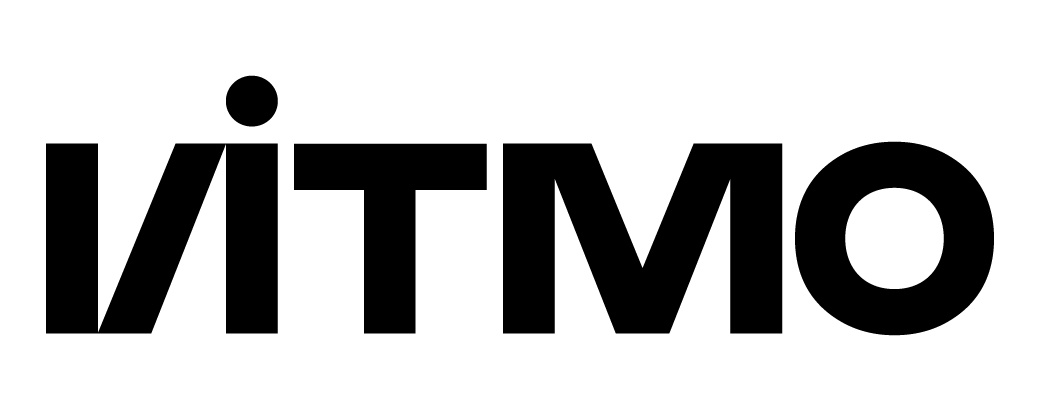
\includegraphics[width=\textwidth]{logo.png}
    % LAB INFO
    {
        \Large
        \textbf{Домашнее задание по теории графов №5}
        \par
        \normalsize
        \vspace*{0.75cm}
        \textbf{Вариант 92}
        \par
    }
    \vfill
    % СREDITS
    \hfill\begin{minipage}{\dimexpr\textwidth-7.8cm}
        \textbf{Выполнил:}\par
        Степанов Арсений Алексеевич\par
        \vspace*{0.15cm}
        \textbf{Группа:}\par
        P3109\par
        \vspace*{0.15cm}
        \textbf{Преподаватель:}\par
        Поляков Владимир Иванович\par
    \end{minipage}
    \vfill
    Санкт-Петербург, \the\year{}г.
\end{titlepage}  
\onehalfspacing
\section*{Матрица смежности графа $G_1$}
\begin{tabular}{|c|c|c|c|c|c|c|c|c|c|c|c|c|c|}
    \hline
    V/V & $e_{1}$ & $e_{2}$ & $e_{3}$ & $e_{4}$ & $e_{5}$ & $e_{6}$ & $e_{7}$ & $e_{8}$ & $e_{9}$ & $e_{10}$ & $e_{11}$ & $e_{12}$ \\
    \hline
    $e_{1}$  & 0 &   &   & 5 &   &   &   & 4 & 1 & 4 &   & 1 \\
    \hline
    $e_{2}$  &   & 0 &   &   & 4 &   & 4 &   & 1 &   &   &   \\
    \hline
    $e_{3}$  &   &   & 0 & 5 &   & 4 & 3 & 4 &   & 3 & 3 &   \\
    \hline
    $e_{4}$  & 5 &   & 5 & 0 &   &   & 1 &   &   &   &   & 1 \\
    \hline
    $e_{5}$  &   & 4 &   &   & 0 & 4 & 4 &   &   &   &   & 5 \\
    \hline
    $e_{6}$  &   &   & 4 &   & 4 & 0 & 5 &   & 3 &   &   & 2 \\
    \hline
    $e_{7}$  &   & 4 & 3 & 1 & 4 & 5 & 0 & 2 &   &   & 5 &   \\
    \hline
    $e_{8}$  & 4 &   & 4 &   &   &   & 2 & 0 &   &   & 1 &   \\
    \hline
    $e_{9}$  & 1 & 1 &   &   &   & 3 &   &   & 0 & 4 & 4 &   \\
    \hline
    $e_{10}$ & 4 &   & 3 &   &   &   &   &   & 4 & 0 & 5 & 5 \\
    \hline
    $e_{11}$ &   &   & 3 &   &   &   & 5 & 1 & 4 & 5 & 0 & 2 \\
    \hline
    $e_{12}$ & 1 &   &   & 1 & 5 & 2 &   &   &   & 5 & 2 & 0 \\
    \hline
\end{tabular}
\section*{Матрица смежности графа $G_2$}
\begin{tabular}{|c|c|c|c|c|c|c|c|c|c|c|c|c|c|}
    \hline
    V/V & $e_{1}$ & $e_{2}$ & $e_{3}$ & $e_{4}$ & $e_{5}$ & $e_{6}$ & $e_{7}$ & $e_{8}$ & $e_{9}$ & $e_{10}$ & $e_{11}$ & $e_{12}$ \\
    \hline
    $e_{1}$  & 0 &   & 3 & 4 &   &   &   & 4 & 2 &   & 5 &   \\
    \hline
    $e_{2}$  &   & 0 & 1 &   &   &   &   & 4 &   &   & 4 &   \\
    \hline
    $e_{3}$  & 3 & 1 & 0 &   & 4 & 4 &   &   &   & 1 &   &   \\
    \hline
    $e_{4}$  & 4 &   &   & 0 & 3 & 3 & 4 &   &   &   & 3 & 5 \\
    \hline
    $e_{5}$  &   &   & 4 & 3 & 0 & 5 & 1 &   & 2 &   & 5 &   \\
    \hline
    $e_{6}$  &   &   & 4 & 3 & 5 & 0 &   &   & 5 & 4 &   &   \\
    \hline
    $e_{7}$  &   &   &   & 4 & 1 &   & 0 &   &   & 4 & 2 &   \\
    \hline
    $e_{8}$  & 4 & 4 &   &   &   &   &   & 0 & 5 &   & 4 &   \\
    \hline
    $e_{9}$  & 2 &   &   &   & 2 & 5 &   & 5 & 0 & 1 &   & 1 \\
    \hline
    $e_{10}$ &   &   & 1 &   &   & 4 & 4 &   & 1 & 0 &   & 5 \\
    \hline
    $e_{11}$ & 5 & 4 &   & 3 & 5 &   & 2 & 4 &   &   & 0 & 1 \\
    \hline
    $e_{12}$ &   &   &   & 5 &   &   &   &   & 1 & 5 & 1 & 0 \\
    \hline
\end{tabular}
\section*{Проверка изоморфности графов}
$\sum\rho_{G_1}(x)=60$, $P(x)=\{7,6,6,6,5,5,5,5,4,4,4,3\}$\\
$\sum\rho_{G_2}(x)=60$, $P(y)=\{7,6,6,6,5,5,5,5,4,4,4,3\}$\\
\hfill\break
Сопоставим вершины графа $G_1$, вершинам графа $G_2$:\\
\hfill\break
\begin{tabular}{|c|c|c|c|c|c|}
    \hline
    $\rho$ & 7 & 6 & 5 & 4 & 3 \\
    \hline
    $P(x)$ & $x_7$ & $x_3$, $x_{11}$, $x_{12}$ & $x_1$, $x_6$, $x_9$, $x_{10}$ & $x_4$, $x_5$, $x_8$ & $x_2$ \\
    \hline
    $P(y)$ & $y_{11}$ & $y_4$, $y_5$, $y_9$ & $y_1$, $y_3$, $y_6$, $y_{10}$ & $y_7$, $y_8$, $y_{12}$ & $y_2$ \\
    \hline
\end{tabular}\\
\\
Получаем следующее соответствие между вершинами графов:\\
\hfill\break
\begin{tabular}{|c|c|}
    \hline
    $P(x)$ & $P(y)$ \\
    \hline
    $x_2$ & $y_2$ \\
    \hline
    $x_7$ & $y_{11}$ \\
    \hline
\end{tabular}\\
\hfill\break
Для определения соответствия вершин с $\rho=4$ проанализируем их связи с неустановленными вершинами\\
$x_4-\{x_1,x_3,x_{12}\}$\\
$x_5-\{x_6,x_{12}\}$\\
$x_8-\{x_1,x_3,x_{11}\}$\\
$y_7-\{y_4,y_5,y_{10}\}$\\
$y_8-\{y_1,y_9\}$\\
$y_{12}-\{y_4,y_9,y_{10}\}$\\
Проанализировав, получаем: \\
\hfill\break
\begin{tabular}{|c|c|}
    \hline
    $P(x)$ & $P(y)$ \\
    \hline
    $x_{3}$ & $y_4$ \\
    \hline
    $x_{5}$ & $y_8$ \\
    \hline
    $x_6$ & $y_1$ \\
    \hline
    $x_{11}$ & $y_5$ \\
    \hline
    $x_{12}$ & $y_9$ \\
    \hline
    \hline
    $x_2$ & $y_2$ \\
    \hline
    $x_7$ & $y_{11}$ \\
    \hline
\end{tabular}\\
\hfill\break
Продолжим анализ для вершин с $\rho=5$\\
$x_1-\{x_4,x_8,x_9,x_{10}\}$\\
$x_6-\{x_9\}$\\
$x_9-\{x_1,x_6,x_{10}\}$\\
$x_{10}-\{x_1,x_9\}$\\
$y_1-\{y_3\}$\\
$y_3-\{y_1,y_6,y_{10}\}$\\
$y_6-\{y_3,y_{10}\}$\\
$y_{10}-\{y_3,y_6,y_7,y_{12}\}$\\
\\\\\\\\\\\\\\\\\\
Проанализировав, получаем: \\
\hfill\break
\begin{tabular}{|c|c|}
    \hline
    $P(x)$ & $P(y)$ \\
    \hline
    $x_1$ & $y_{10}$ \\
    \hline
    $x_9$ & $y_3$ \\
    \hline
    $x_{10}$ & $y_6$ \\
    \hline
    \hline
    $x_2$ & $y_2$ \\
    \hline
    $x_3$ & $y_4$ \\
    \hline
    $x_{5}$ & $y_8$ \\
    \hline
    $x_6$ & $y_1$ \\
    \hline
    $x_7$ & $y_{11}$ \\
    \hline
    $x_{11}$ & $y_5$ \\
    \hline
    $x_{12}$ & $y_9$ \\
    \hline
\end{tabular}\\
\hfill\break
Проанализируем оставшиеся вершины: \\
$x_4-\{x_{12}\}$\\
$x_8-\{x_{11}\}$\\
$y_7-\{y_5\}$\\
$y_{12}-\{y_9\}$\\
Проанализировав, получаем: \\
\hfill\break
\begin{tabular}{|c|c|}
    \hline
    $P(x)$ & $P(y)$ \\
    \hline
    $x_4$ & $y_{12}$ \\
    \hline
    $x_8$ & $y_7$ \\
    \hline
    \hline
    $x_1$ & $y_{10}$ \\
    \hline
    $x_2$ & $y_2$ \\
    \hline
    $x_3$ & $y_4$ \\
    \hline
    $x_{5}$ & $y_8$ \\
    \hline
    $x_6$ & $y_1$ \\
    \hline
    $x_7$ & $y_{11}$ \\
    \hline
    $x_9$ & $y_3$ \\
    \hline
    $x_{10}$ & $y_6$ \\
    \hline
    $x_{11}$ & $y_5$ \\
    \hline
    $x_{12}$ & $y_9$ \\
    \hline
\end{tabular}\\
\hfill\break
Каждой из вершин графа $G_1$ можно сопоставить вершину графа $G_2$, следовательно, они изоморфны
\end{document}

$x_4-\{x_1,x_3\}$\\
$x_5-\{x_2,x_6\}$\\
$x_8-\{x_1,x_3\}$\\
$x_3-\{4,6,7,8,{10},{11}\}$

$y_7-\{y_4,y_{10}\}$\\
$y_8-\{y_1,y_2\}$\\
$y_{12}-\{y_4,y_{10}\}$\\

